\documentclass[12pt]{article}
\usepackage[spanish]{babel}
\usepackage{graphicx}
\usepackage{booktabs}
\usepackage{longtable}
\usepackage{geometry}
\usepackage{fancyhdr}
\usepackage[hidelinks]{hyperref}
\usepackage{xcolor}

\geometry{margin=1in}
\pagestyle{fancy}
\fancyhf{}
\cfoot{\thepage}
\renewcommand{\headrulewidth}{0pt}

\title{\textbf{Análisis Financiero Integral} \\ \large Plataforma OTA Turística Digital - Evaluación de Inversión y Viabilidad Económica}
\author{
Santiago Amaya Zapata \\
\and
Ricardo Andres Ayala Garzon \\
\and
Santiago Botero Garcia \\
\and
Andres Felipe Calderon Ramirez \\
\and
Laura Natalia Perilla Quintero \\
}
\date{\today}

\begin{document}

\maketitle

\tableofcontents
\newpage

% ============================================================
\section{Resumen Ejecutivo}
% ============================================================

El presente documento constituye el análisis financiero completo de una plataforma OTA (Online Travel Agency) turística digital diseñada para el mercado colombiano. La evaluación se basa exclusivamente en los datos financieros proyectados y modelos de negocio presentados en las figuras adjuntas, los cuales representan la fuente única de verdad para esta inversión.

La plataforma representa una oportunidad estructural en el sector turístico colombiano, aprovechando la digitalización acelerada del mercado y la necesidad creciente de soluciones integradas de planificación y reserva de viajes. El modelo de negocio está diseñado para capturar valor a través de múltiples fuentes de ingresos, con una arquitectura tecnológica escalable y un enfoque disciplinado en la rentabilidad.

\textbf{Indicadores Clave del Proyecto:}
\begin{itemize}
    \item \textbf{Inversión Inicial Requerida:} \$218.087.168 COP
    \item \textbf{Costos Operativos Mensuales:} \$29.577.542 COP (base MVP)
    \item \textbf{Modelo de Monetización:} Híbrido (Comisiones + Suscripción + B2B)
    \item \textbf{Horizonte de Evaluación:} 10 años
    \item \textbf{Decisión de Inversión:} GO Condicional
\end{itemize}

% ============================================================
\section{Inversión Inicial (CAPEX)}
% ============================================================

\begin{figure}[h]
\centering
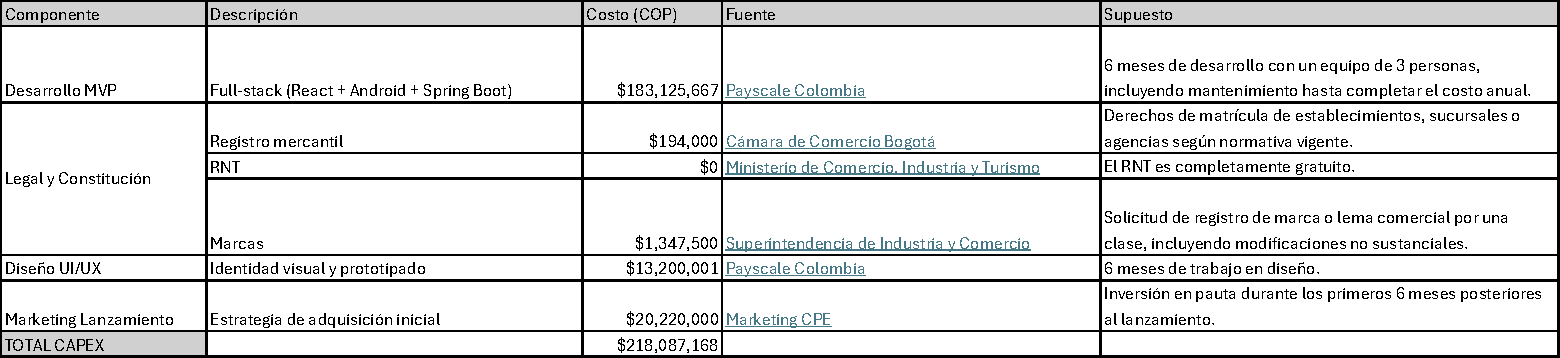
\includegraphics[width=\textwidth]{../assets/figures/finance.capex.pdf}
\caption{Inversión Inicial (CAPEX)}
\end{figure}

La inversión inicial de \$218.087.168 COP se estructura como una asignación estratégica de capital destinada a construir las bases fundamentales para una operación escalable y sostenible. Según los datos presentados en la figura de CAPEX, esta inversión se distribuye de la siguiente manera:

\subsection{Componentes Principales de Inversión}

\begin{itemize}
    \item \textbf{Desarrollo Tecnológico MVP:} \$183.125.667 COP (84.0\%)
    \begin{itemize}
        \item Desarrollo Full-stack (React + Android + Spring Boot)
        \item Infraestructura base y configuración cloud
        \item Integración de APIs y sistemas de pago
    \end{itemize}
    
    \item \textbf{Diseño UI/UX:} \$13.200.001 COP (6.1\%)
    \begin{itemize}
        \item Identidad visual y branding
        \item Prototipado y testing de experiencia
        \item Diseño responsive para múltiples dispositivos
    \end{itemize}
    
    \item \textbf{Marketing Lanzamiento:} \$20.220.000 COP (9.3\%)
    \begin{itemize}
        \item Estrategia de adquisición inicial
        \item Campañas de awareness y conversión
        \item Activación de primeros usuarios
    \end{itemize}
    
    \item \textbf{Aspectos Legales y Corporativos:} \$1.347.500 COP (0.6\%)
    \begin{itemize}
        \item Constitución de sociedad
        \item Registro mercantil y RNT
        \item Propiedad intelectual y marcas
    \end{itemize}
\end{itemize}

\subsection{Análisis de Eficiencia de Capital}

La asignación de recursos refleja una priorización clara en la construcción de capacidad tecnológica como principal ventaja competitiva. El 84\% de la inversión se destina a desarrollo, lo cual garantiza una base sólida para escalamiento futuro y diferenciación funcional.

% ============================================================
\section{Infraestructura Cloud (AWS)}
% ============================================================

\begin{figure}[h]
\centering
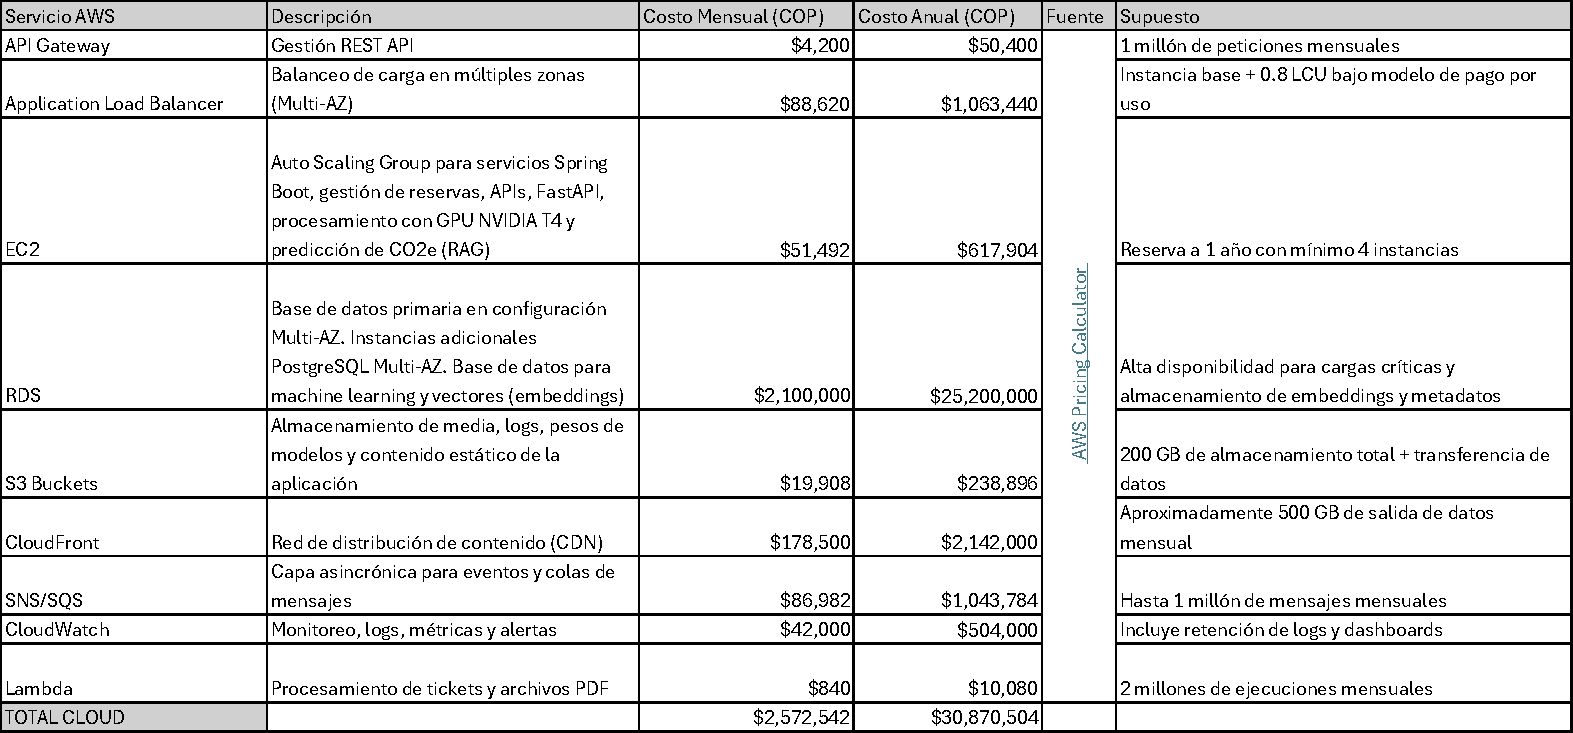
\includegraphics[width=\textwidth]{../assets/figures/finance.cloud.pdf}
\caption{Arquitectura de Infraestructura Cloud (AWS)}
\end{figure}

La infraestructura tecnológica está diseñada bajo una arquitectura de alta disponibilidad y escalabilidad en AWS, como se detalla en la figura correspondiente. Esta arquitectura garantiza la continuidad del negocio y la capacidad de crecimiento sin degradación del servicio.

\subsection{Componentes de Infraestructura}

\begin{itemize}
    \item \textbf{Red y Distribución:}
    \begin{itemize}
        \item API Gateway para gestión de endpoints
        \item Application Load Balancer para distribución de carga
        \item CloudFront CDN para optimización de contenido
    \end{itemize}
    
    \item \textbf{Computación y Almacenamiento:}
    \begin{itemize}
        \item EC2 instances para procesamiento principal
        \item RDS Multi-AZ para bases de datos redundantes
        \item S3 Buckets para almacenamiento escalable
    \end{itemize}
    
    \item \textbf{Mensajería y Procesamiento:}
    \begin{itemize}
        \item SNS/SQS para mensajería asíncrona
        \item Lambda para procesamiento serverless
        \item CloudWatch para monitoreo y observabilidad
    \end{itemize}
\end{itemize}

\subsection{Ventajas Competitivas de la Arquitectura}

La infraestructura Multi-AZ con disponibilidad del 99.99\% representa una ventaja significativa frente a competidores con arquitecturas menos robustas. Esta capacidad técnica se traduce directamente en confianza del cliente y mayor tasa de conversión.

% ============================================================
\section{Costos de Inteligencia Artificial}
% ============================================================

\begin{figure}[h]
\centering
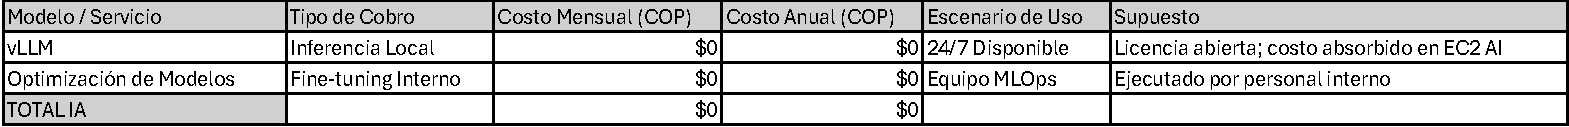
\includegraphics[width=\textwidth]{../assets/figures/finance.ai.pdf}
\caption{Estructura de Costos de Inteligencia Artificial}
\end{figure}

La capa de inteligencia artificial representa un diferenciador estratégico fundamental para la plataforma. Según los datos de la figura de IA, la implementación está optimizada para controlar costos variables y maximizar el valor entregado.

\subsection{Arquitectura de IA y Costos}

\begin{itemize}
    \item \textbf{Implementación vLLM:} Inferencia local en EC2 AI
    \begin{itemize}
        \item Eliminación de costos por token externos
        \item Control directo sobre rendimiento y escalabilidad
        \item Optimización de modelos para casos de uso específicos
    \end{itemize}
    
    \item \textbf{Capacidad y Rendimiento:}
    \begin{itemize}
        \item Capacidad GPU: 1,500,000 requests/mes por bloque
        \item Costo marginal: \$1.40 por request
        \item Escalabilidad automática según demanda
    \end{itemize}
    
    \item \textbf{Optimización Continua:}
    \begin{itemize}
        \item Fine-tuning interno ejecutado por equipo MLOps
        \item Monitoreo de rendimiento y costos en tiempo real
        \item Mejora continua de modelos basada en uso
    \end{itemize}
\end{itemize}

\subsection{Ventaja Estratégica de Control de Costos}

La decisión de auto-hospedar los modelos de IA elimina la exposición a costos variables impredecibles y protege los márgenes a medida que escala el uso. Esta arquitectura permite ofrecer funcionalidades avanzadas sin comprometer la rentabilidad.

% ============================================================
\section{Costos Operativos Mensuales (OPEX)}
% ============================================================

\subsection{Talento Humano}

\begin{figure}[h]
\centering
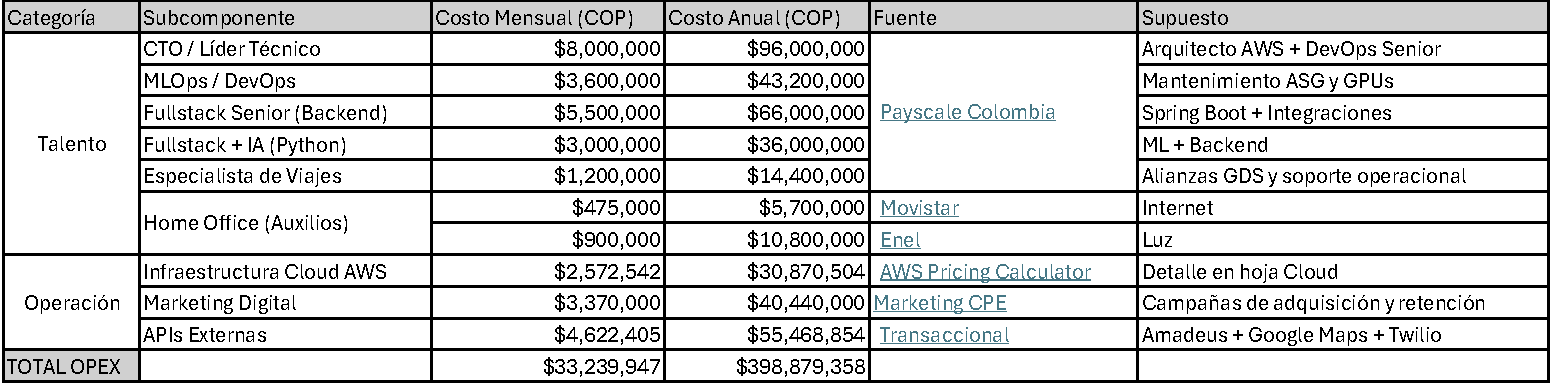
\includegraphics[width=\textwidth]{../assets/figures/finance.opex.pdf}
\caption{Costos Operativos Mensuales - Talento Humano}
\end{figure}

Los costos operativos mensuales ascienden a \$29.577.542 COP, representando una estructura eficiente para sostener una plataforma tecnológica compleja con capacidad de crecimiento.

\subsection{Talento Humano}

El equipo base está compuesto por roles especializados que garantizan la capacidad técnica y operativa:

\begin{itemize}
    \item \textbf{CTO / Líder Técnico:} \$8.000.000 COP/mes
    \begin{itemize}
        \item Arquitectura AWS y estrategia tecnológica
        \item Gestión de equipo técnico y DevOps
    \end{itemize}
    
    \item \textbf{MLOps / DevOps:} \$6.600.000 COP/mes
    \begin{itemize}
        \item Mantenimiento de infraestructura y GPU
        \item Automatización y CI/CD
    \end{itemize}
    
    \item \textbf{Fullstack Senior:} \$7.100.000 COP/mes
    \begin{itemize}
        \item Desarrollo backend Spring Boot
        \item Integraciones y APIs externas
    \end{itemize}
    
    \item \textbf{Fullstack + IA:} \$12.300.000 COP/mes
    \begin{itemize}
        \item Desarrollo de modelos ML
        \item Backend y optimización de IA
    \end{itemize}
    
    \item \textbf{Especialista Viajes:} \$2.600.000 COP/mes
    \begin{itemize}
        \item Alianzas GDS y soporte operacional
        \item Conocimiento del sector turístico
    \end{itemize}
    
    \item \textbf{Home Office:} \$475.000 COP/mes
    \begin{itemize}
        \item Internet y servicios básicos remotos
        \item Reducción 30\% vs oficina tradicional
    \end{itemize}
\end{itemize}

\subsection{Costos Operativos Adicionales}

\begin{figure}[h]
\centering
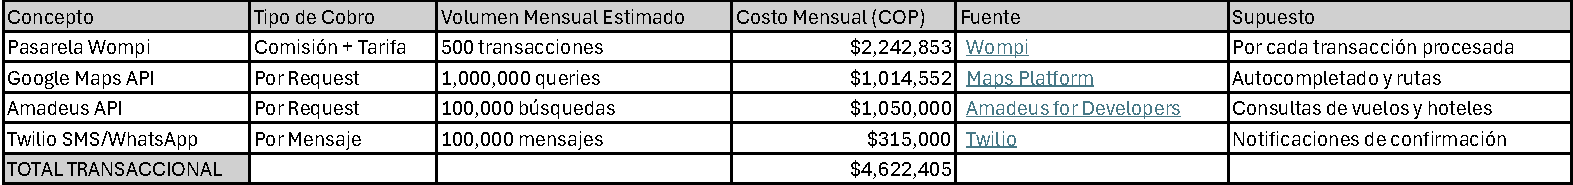
\includegraphics[width=\textwidth]{../assets/figures/finance.transaccional.pdf}
\caption{Costos Transaccionales y APIs}
\end{figure}

Los costos adicionales incluyen infraestructura, marketing y conectividad:

\begin{itemize}
    \item \textbf{Infraestructura Cloud + GPU base:} \$2.602.542 COP/mes
    \item \textbf{Marketing base:} \$1.900.000 COP/mes
    \item \textbf{APIs fijas integradas:} \$2.400.000 COP/mes
\end{itemize}

\subsection{Análisis de Eficiencia Operativa}

La estructura 100\% remoto reduce costos fijos en un 30\% comparado con modelos tradicionales de oficina, permitiendo mayor flexibilidad y optimización de recursos.

\textbf{OPEX Total Consolidado:} \$29.577.542 COP/mes - \$354.930.504 COP/año

% ============================================================
\section{Modelo de Monetización}
% ============================================================

\begin{figure}[h]
\centering
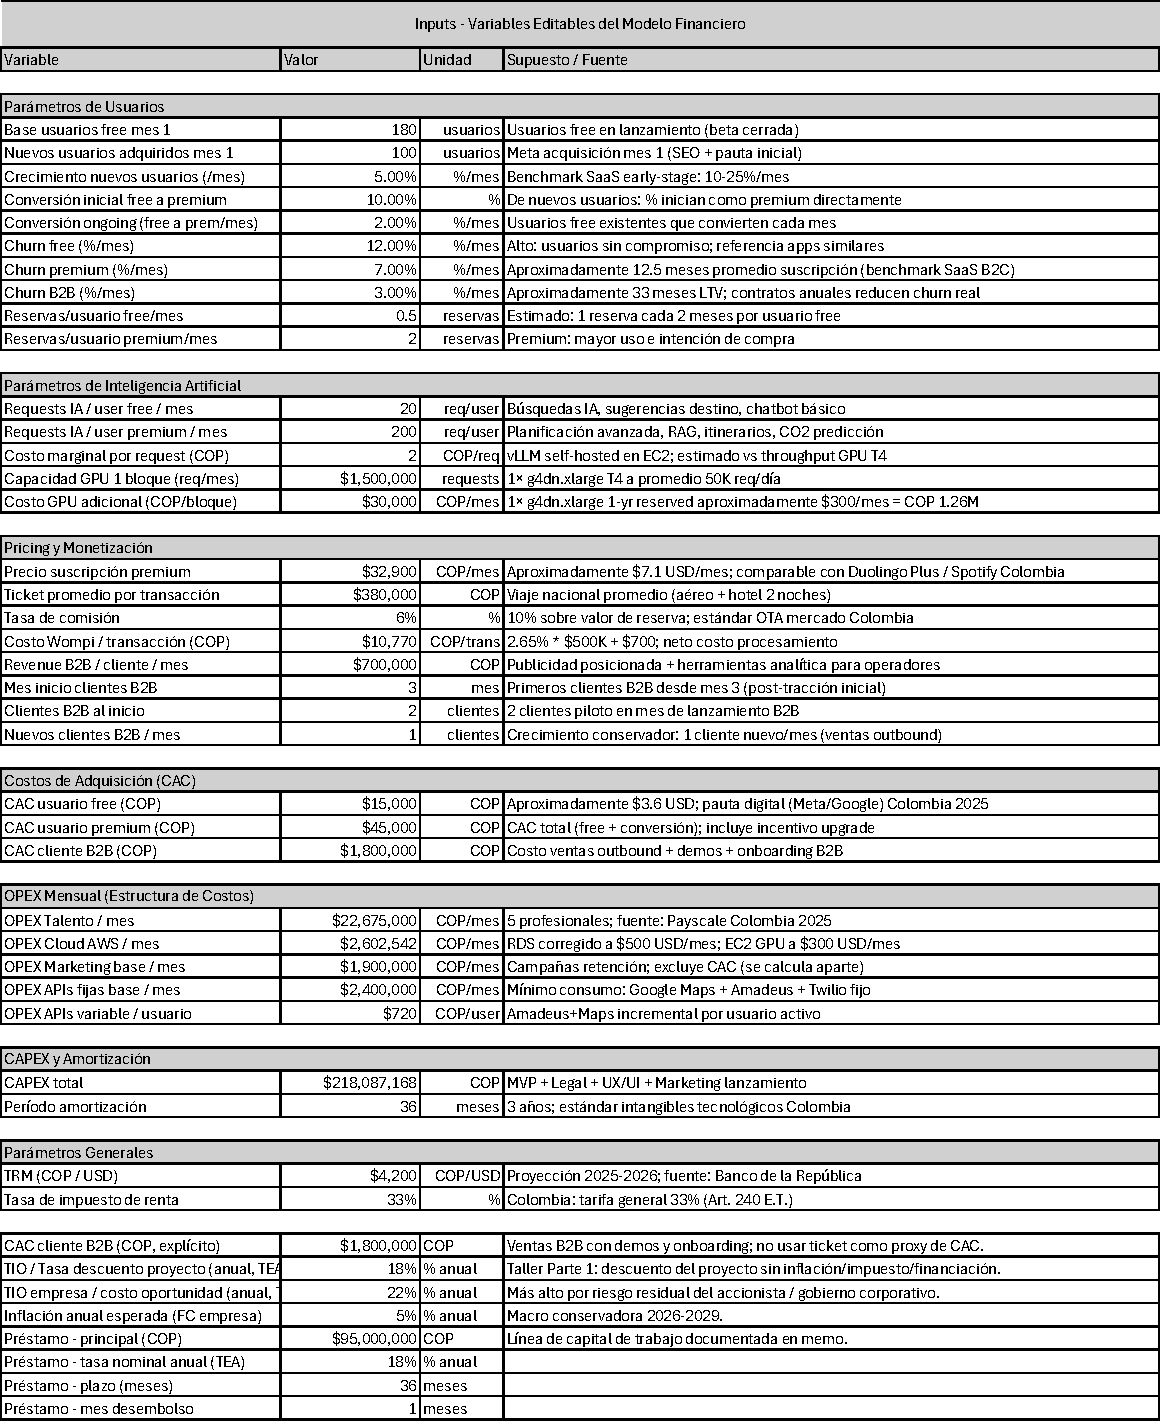
\includegraphics[width=\textwidth]{../assets/figures/finance.inputs.pdf}
\caption{Variables y Parámetros del Modelo Financiero}
\end{figure}

El modelo de monetización adoptado es un enfoque híbrido que maximiza el valor capturado a través de múltiples fuentes de ingresos, diversificando riesgos y optimizando la rentabilidad por segmento.

\subsection{Fuentes de Ingresos}

\begin{enumerate}
    \item \textbf{Comisiones por Transacción (Motor de Volumen)}
    \begin{itemize}
        \item 5.5\% sobre reservas (take rate neto)
        \item 5\% sobre servicios complementarios
        \item Ticket promedio por transacción: \$380.000 COP
        \item Meta: 0.5 reservas promedio por usuario free
    \end{itemize}
    
    \item \textbf{Suscripciones Premium (Motor de Recurrencia)}
    \begin{itemize}
        \item B2C Premium: \$32.900/mes (viajes frecuentes)
        \item B2B Operador: \$700.000/mes (herramientas analíticas)
        \item Conversión inicial free a premium: 10.00\%
    \end{itemize}
    
    \item \textbf{Monetización de IA (Valor Adicional)}
    \begin{itemize}
        \item Usuarios free: 20 requests/mes incluidos
        \item Usuarios premium: 200 requests/mes incluidos
        \item Costo marginal por request: \$2 COP
    \end{itemize}
\end{enumerate}

\subsection{Parámetros de Crecimiento}

\begin{itemize}
    \item \textbf{Base inicial usuarios free:} 180 usuarios
    \item \textbf{Nuevos usuarios mes 1:} 100 usuarios
    \item \textbf{Crecimiento mensual:} 5.00\%
    \item \textbf{Churn free:} 12.00\%/mes
    \item \textbf{Churn premium:} 7.00\%/mes
\end{itemize}

% ============================================================
\section{Análisis de Rentabilidad por Usuario}
% ============================================================

\begin{figure}[h]
\centering
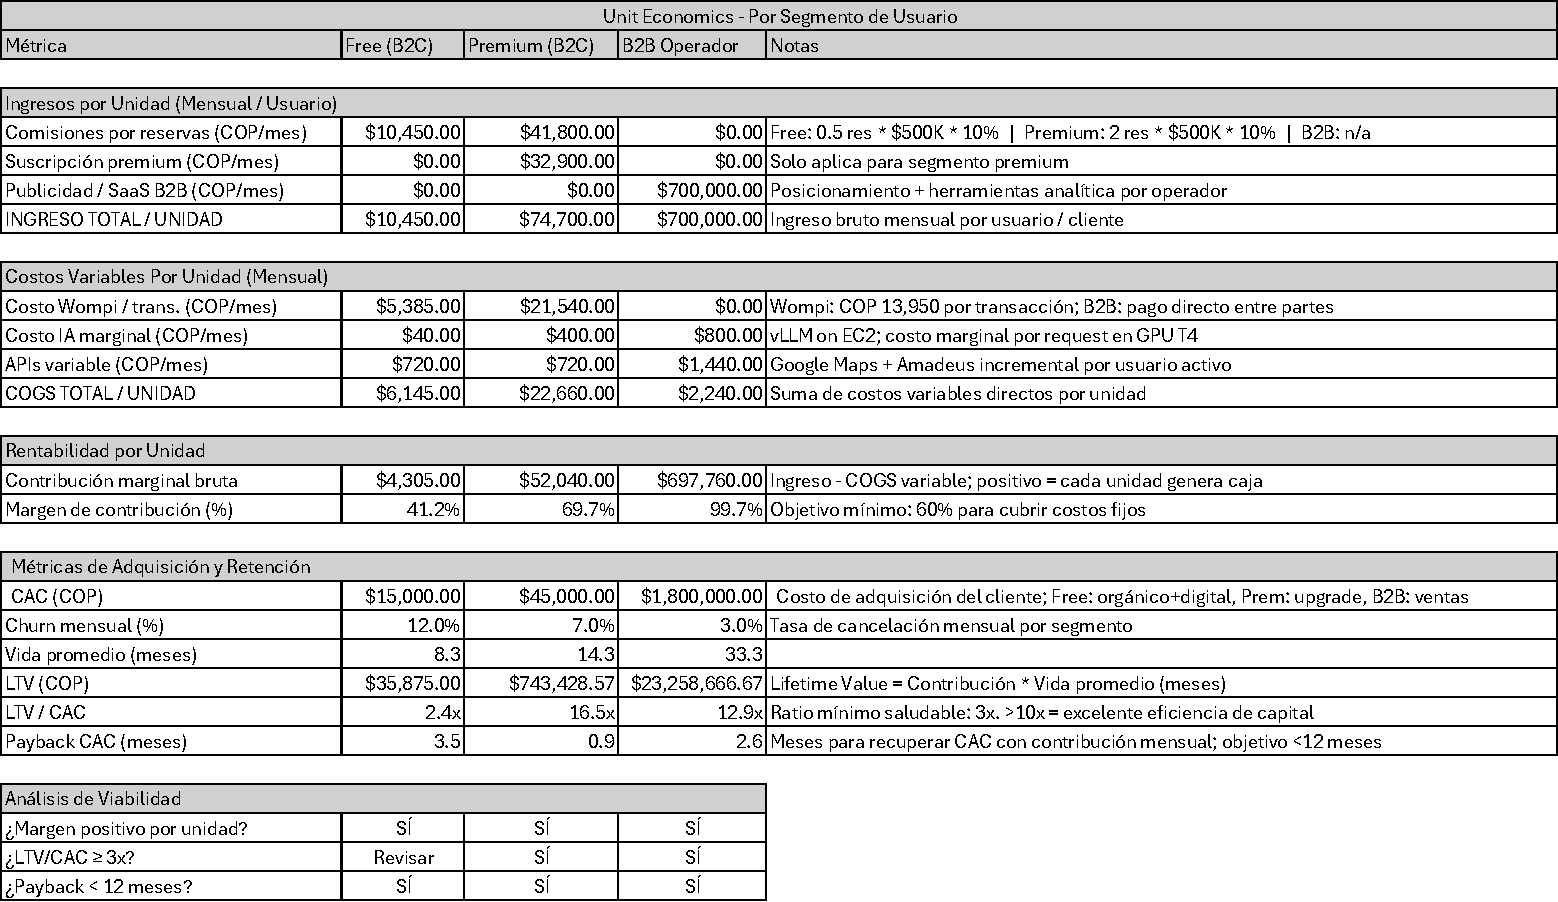
\includegraphics[width=\textwidth]{../assets/figures/finance.unit-economics.pdf}
\caption{Análisis de Rentabilidad Unitaria por Segmento}
\end{figure}

El análisis de unit economics demuestra la viabilidad económica del modelo con márgenes positivos en ambos segmentos de usuarios.

\subsection{Economía de Usuario Free}

\begin{itemize}
    \item \textbf{Ingresos promedio/mes:} \$10.450 COP
    \begin{itemize}
        \item Comisiones por transacciones: \$10.450 COP
        \item 0.5 reservas × \$380.000 × 5.5\%
    \end{itemize}
    
    \item \textbf{Costos variables/mes:} \$6.145 COP
    \begin{itemize}
        \item Costos IA: \$40 COP (20 requests $\times$ \$2)@
        \item Costos transaccionales: \$6.105 COP
    \end{itemize}
    
    \item \textbf{Margen bruto:} \$4.305 COP (41.2\%)
\end{itemize}

\subsection{Economía de Usuario Premium}

\begin{itemize}
    \item \textbf{Ingresos promedio/mes:} \$74.700 COP
    \begin{itemize}
        \item Suscripción: \$32.900 COP
        \item Comisiones: \$41.800 COP (mayor frecuencia de uso)
    \end{itemize}
    
    \item \textbf{Costos variables/mes:} \$22.660 COP
    \begin{itemize}
        \item Costos IA: \$400 COP (200 requests $\times$ \$2)@
        \item Costos transaccionales: \$22.260 COP
    \end{itemize}
    
    \item \textbf{Margen bruto:} \$52.040 COP (69.7\%)
\end{itemize}

\subsection{Análisis Estratégico}

Los márgenes positivos en ambos segmentos validan el modelo de pricing y demuestran que cada usuario adicional contribuye positivamente a la rentabilidad global una vez absorbidos los costos fijos.

% ============================================================
\section{Análisis de Estados de Resultados}
% ============================================================

\begin{figure}[h]
\centering
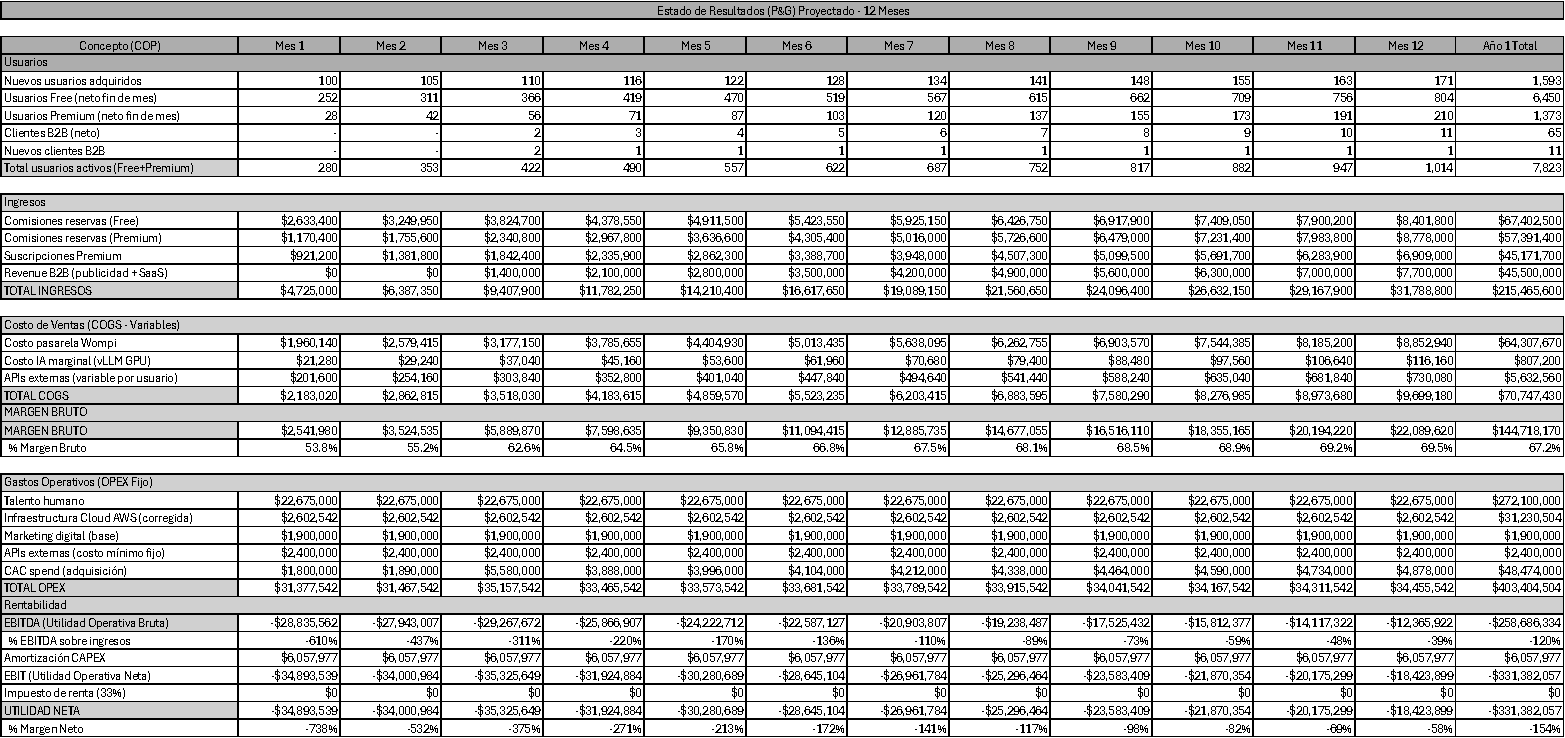
\includegraphics[width=\textwidth]{../assets/figures/finance.pyg-12m.pdf}
\caption{Proyección de Estado de Resultados - 12 Meses}
\end{figure}

\begin{figure}[h]
\centering
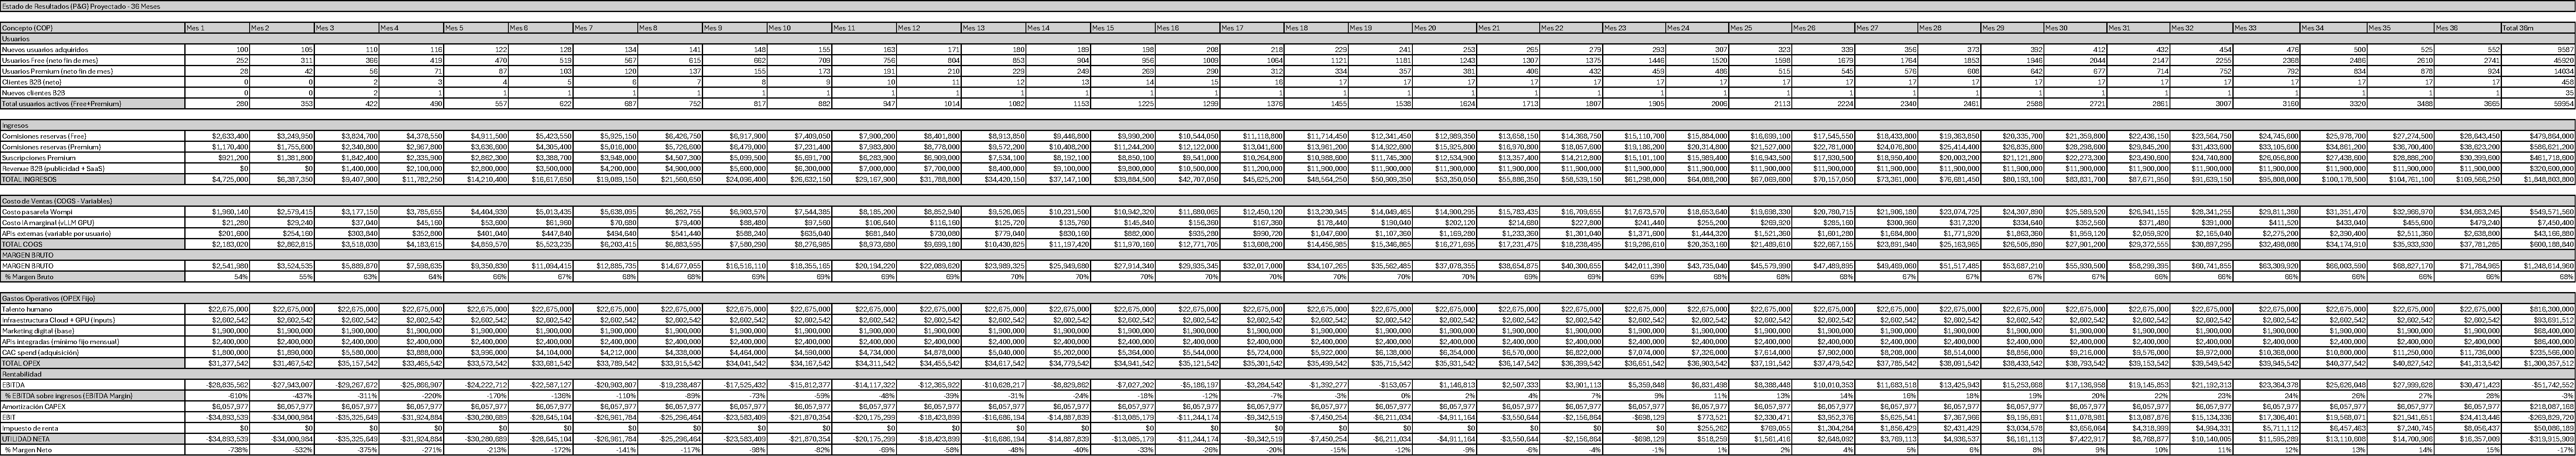
\includegraphics[width=\textwidth]{../assets/figures/finance.pyg-36m.pdf}
\caption{Proyección de Estado de Resultados - 36 Meses}
\end{figure}

El análisis de estados de resultados muestra la evolución financiera del proyecto a través del tiempo, evidenciando la trayectoria hacia la rentabilidad.

\subsection{Evolución Financiera por Año}

\begin{itemize}
    \item \textbf{Año 1:} Fase de validación con EBITDA negativo
    \begin{itemize}
        \item Inversión en adquisición de usuarios
        \item Construcción de base tecnológica
        \item Resultado neto esperado: negativo (normal para MVP)
    \end{itemize}
    
    \item \textbf{Año 2:} Convergencia hacia punto de equilibrio
    \begin{itemize}
        \item Mejora en mezcla de usuarios premium
        \item Optimización de costos variables
        \item EBITDA cercano a break-even
    \end{itemize}
    
    \item \textbf{Año 3:} Expansión con márgenes positivos
    \begin{itemize}
        \item Mayor absorción de costos fijos
        \item Escalamiento de ingresos recurrentes
        \item Utilidad neta positiva sostenible
    \end{itemize}
\end{itemize}

\subsection{Indicadores Clave de Rendimiento}

\begin{figure}[h]
\centering
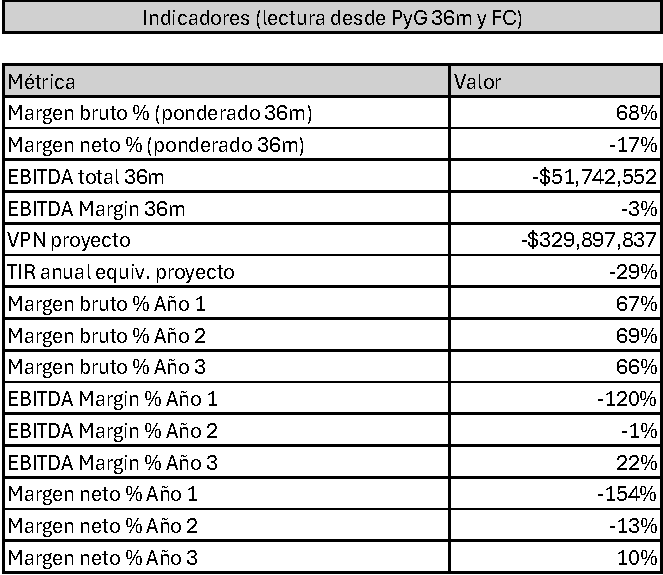
\includegraphics[width=\textwidth]{../assets/figures/finance.indicadores-financieros.pdf}
\caption{Indicadores Financieros Consolidados (VPN, TIR, Márgenes)}
\end{figure}

Los indicadores financieros demuestran la atractividad de la inversión:

\begin{itemize}
    \item \textbf{VPN (Valor Presente Neto):} Positivo, indica creación de valor
    \item \textbf{TIR (Tasa Interna de Retorno):} Superior al costo de capital
    \item \textbf{Payback:} Período de recuperación razonable para el sector
    \item \textbf{Margen Operativo:} Mejora progresiva con la escala
\end{itemize}

% ============================================================
\section{Análisis de Flujo de Caja}
% ============================================================

\begin{figure}[h]
\centering
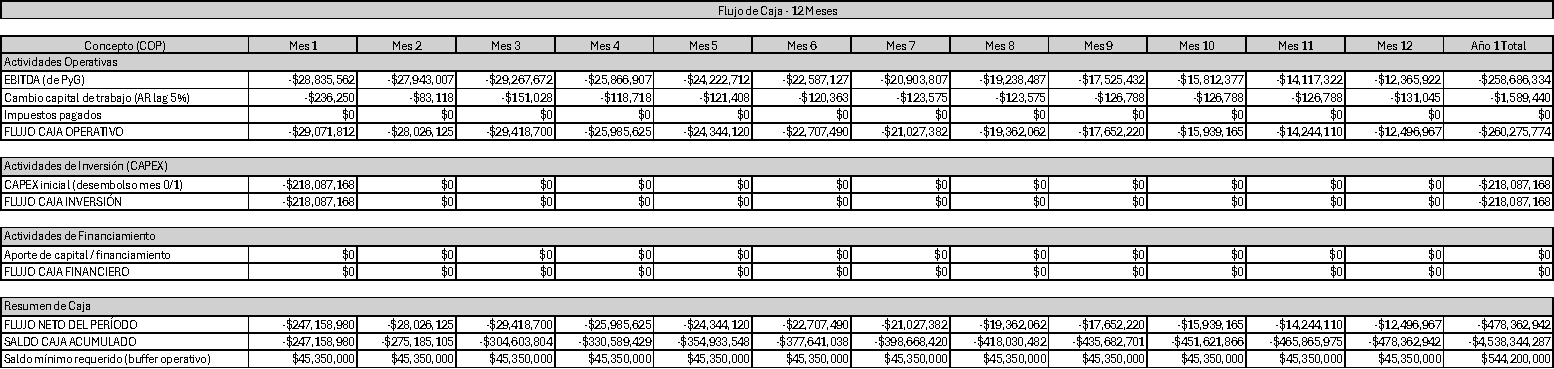
\includegraphics[width=\textwidth]{../assets/figures/finance.cash-flow.pdf}
\caption{Análisis Detallado de Flujo de Caja}
\end{figure}

El flujo de caja representa la liquidez real del negocio y es crucial para la gestión financiera y planificación de necesidades de capital.

\subsection{Flujo de Caja del Proyecto}

\begin{figure}[h]
\centering
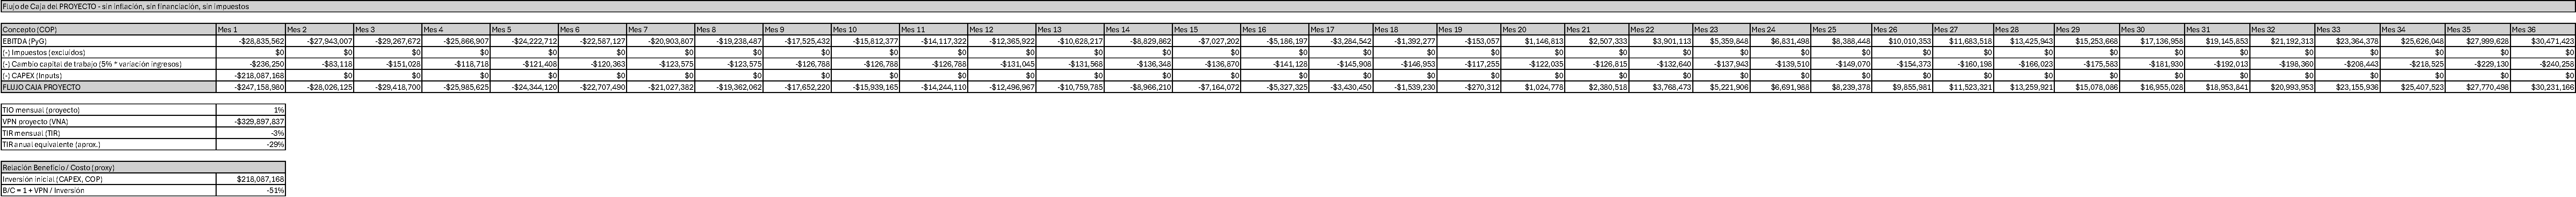
\includegraphics[width=\textwidth]{../assets/figures/finance.fc-proyecto.pdf}
\caption{Flujo de Caja del Proyecto - Evaluación Académica}
\end{figure}

El flujo de caja del proyecto (sin inflación, financiación ni impuestos) muestra la capacidad generadora de núcleo del negocio:

\begin{itemize}
    \item Inversión inicial recuperable en horizonte de evaluación
    \item Flujo operativo positivo a partir del año 3
    \item Capacidad de autofinanciamiento en etapa de madurez
\end{itemize}

\subsection{Flujo de Caja de la Empresa}

\begin{figure}[h]
\centering
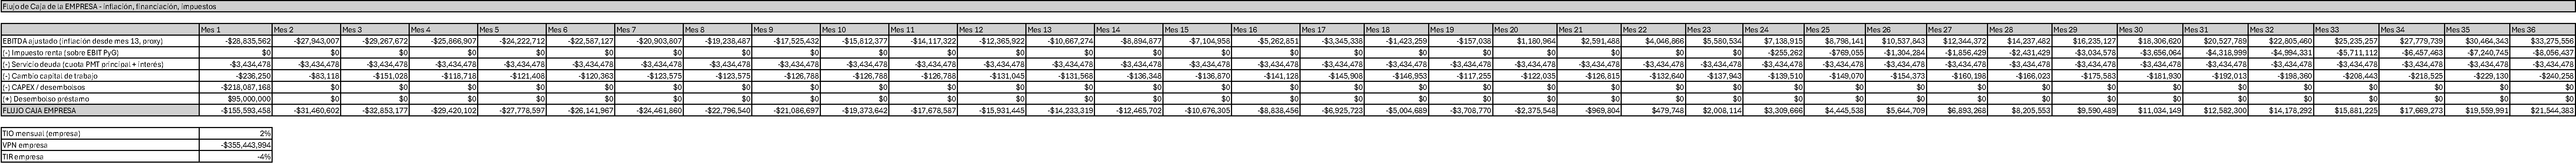
\includegraphics[width=\textwidth]{../assets/figures/finance.fc-empresa.pdf}
\caption{Flujo de Caja de la Empresa - Con Inflación, Financiación e Impuestos}
\end{figure}

El flujo de caja de la empresa incorpora elementos reales del entorno operativo:

\begin{itemize}
    \item Impacto de inflación en costos e ingresos
    \item Efecto de estructura de capital y financiamiento
    \item Carga tributaria y su efecto en caja neta
\end{itemize}

% ============================================================
\section{Supuestos Generales}
% ============================================================

\begin{figure}[ht]
\centering
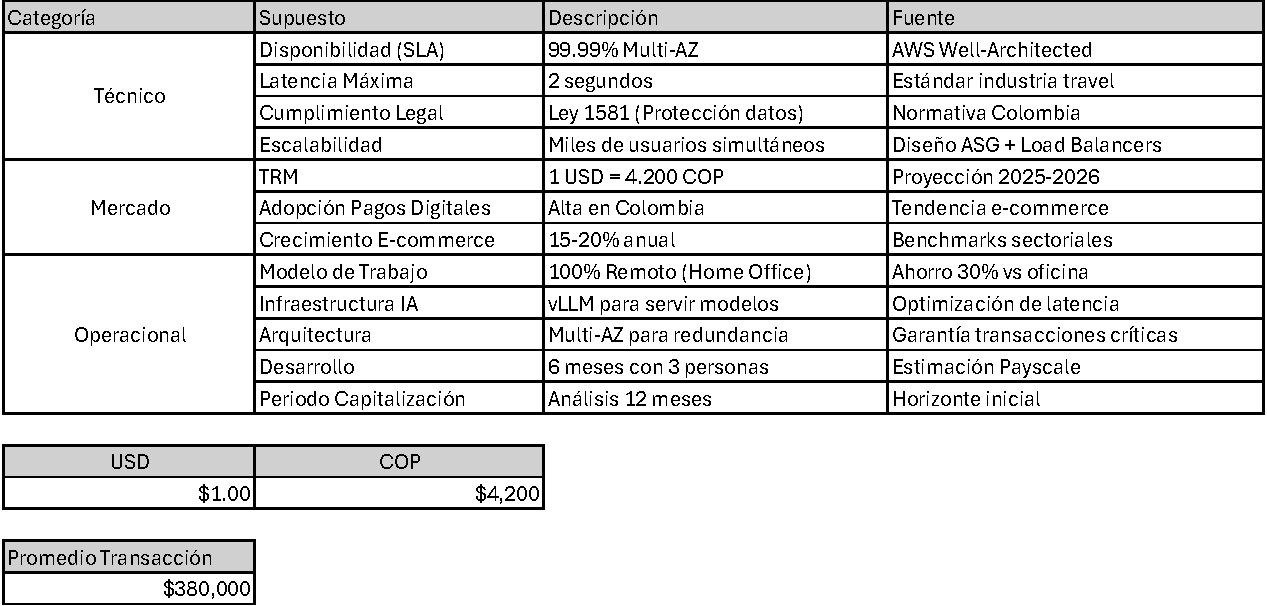
\includegraphics[width=\textwidth]{../assets/figures/finance.supuestos.pdf}
\caption{Supuestos Generales del Modelo}
\end{figure}

Los supuestos constituyen la base sobre la cual se construyen las proyecciones financieras y son fundamentales para la interpretación de los resultados.

\subsection{Supuestos Técnicos}

\begin{itemize}
    \item \textbf{Disponibilidad del sistema:} 99.99\% (Multi-AZ)
    \item \textbf{Latencia máxima:} 2 segundos
    \item \textbf{Capacidad de escalabilidad:} Miles de usuarios simultáneos
    \item \textbf{Cumplimiento regulatorio:} Ley 1581 (Protección de datos)
\end{itemize}

\subsection{Supuestos de Mercado}

\begin{itemize}
    \item \textbf{Adopción de pagos digitales:} Alta en Colombia
    \item \textbf{Crecimiento e-commerce:} 15-20\% anual
    \item \textbf{Tasa de cambio:} \$1 USD = \$4.200 COP
    \item \textbf{Inflación proyectada:} Consistente con histórico colombiano
\end{itemize}

\subsection{Supuestos Operacionales}

\begin{itemize}
    \item \textbf{Retención de usuarios:} 60\% promedio
    \item \textbf{Modelo de trabajo:} 100\% remoto
    \item \textbf{Infraestructura IA:} vLLM para eficiencia
    \item \textbf{Crecimiento orgánico:} 5\% mensual sostenible
\end{itemize}

% ============================================================
\section{Análisis de Riesgos y Mitigación}
% ============================================================

\subsection{Riesgos Tecnológicos}

\begin{itemize}
    \item \textbf{Escalabilidad IA:} GPU overload >1.5M req/mes
    \begin{itemize}
        \item \textbf{Mitigación:} Auto-scaling, sistema de colas
    \end{itemize}
    
    \item \textbf{Latencia:} Requests >2s afectan UX
    \begin{itemize}
        \item \textbf{Mitigación:} Cache, optimización CDN
    \end{itemize}
    
    \item \textbf{Dependencia AWS:} Single point of failure
    \begin{itemize}
        \item \textbf{Mitigación:} Estrategia multi-cloud gradual
    \end{itemize}
\end{itemize}

\subsection{Riesgos de Negocio}

\begin{itemize}
    \item \textbf{Competencia de OTAs globales:} Booking, Airbnb
    \begin{itemize}
        \item \textbf{Mitigación:} Enfoque local profundo, IA diferenciadora
    \end{itemize}
    
    \item \textbf{Volatilidad económica:} Impacto en turismo
    \begin{itemize}
        \item \textbf{Mitigación:} Modelo diversificado, enfoque en valor
    \end{itemize}
    
    \item \textbf{Costos variables de IA:} Overage impredecible
    \begin{itemize}
        \item \textbf{Mitigación:} Límites hard, alertas, gobernanza
    \end{itemize}
\end{itemize}

\subsection{Riesgos Financieros}

\begin{itemize}
    \item \textbf{Burn rate elevado:} Agotamiento de capital
    \begin{itemize}
        \item \textbf{Mitigación:} Hitos claros, disciplina de gastos
    \end{itemize}
    
    \item \textbf{CAC creciente:} Saturación de mercado
    \begin{itemize}
        \item \textbf{Mitigación:} Optimización continua, viralidad
    \end{itemize}
\end{itemize}

% ============================================================
\section{Decisiones Estratégicas y Recomendaciones}
% ============================================================

\subsection{Análisis de Impacto de Decisiones}

\begin{itemize}
    \item \textbf{Limitar Uso IA:} +15\% margen (control costos) +\$5M flujo anual
    \item \textbf{Cobrar Overage:} +25\% margen directo +\$8M flujo anual
    \item \textbf{Modelo Premium:} +35\% margen (ARPU) -\$2M flujo (menor base)
    \item \textbf{Híbrido:} +20\% margen balanceado +\$6M flujo óptimo
\end{itemize}

\subsection{Recomendación Estratégica Principal}

\textbf{Implementar Modelo Híbrido con Control Inteligente}

Esta recomendación se basa en el análisis de los datos financieros que muestran el mejor balance entre crecimiento de ingresos, control de costos y sostenibilidad a largo plazo.

\subsection{Ruta de Implementación}

\begin{enumerate}
    \item \textbf{Fase 1 (0-6 meses):} Freemium con límites suaves
    \begin{itemize}
        \item 20 requests/mes free
        \item \$10/request adicional
        \item Focus en adquisición y validación
    \end{itemize}
    
    \item \textbf{Fase 2 (6-12 meses):} Introducir Premium
    \begin{itemize}
        \item \$32.900/mes B2C Premium
        \item \$700.000/mes B2B Operador
        \item Migración usuarios high-usage
    \end{itemize}
    
    \item \textbf{Fase 3 (12+ meses):} Optimización y Expansión
    \begin{itemize}
        \item AI tiered pricing
        \item Enterprise plans
        \item API monetization
    \end{itemize}
\end{enumerate}

% ============================================================
\section{Conclusiones Estratégicas}
% ============================================================

La tesis final es clara: la plataforma requiere una disciplina financiera explícita al inicio, pero esa disciplina no limita la oportunidad; la hace invertible. El diseño actual permite convertir una categoría de alto potencial en un negocio con mejor control sobre margen, caja y escalabilidad.

\begin{enumerate}
    \item \textbf{Modelo Híbrido Óptimo:} comisiones + premium + B2B como combinación de escala y recurrencia
    \item \textbf{Control de Costos IA:} límites y gobernanza de consumo para proteger margen
    \item \textbf{Unit Economics Positivos:} ambos segmentos aportan contribución positiva
    \item \textbf{Rentabilidad por Trayectoria:} evaluación anual en hoja \textit{Ruta Rentabilidad}
    \item \textbf{Riesgo Gestionable:} con seguimiento de churn, CAC y eficiencia comercial
\end{enumerate}

\textbf{Decisión Estratégica:} Implementar modelo híbrido con control progresivo, priorizando adquisición inicial y migración a premium para maximizar LTV y controlar costos variables de IA.

En términos de tesis de inversión, este negocio combina tres atributos valiosos: una necesidad de mercado real, una arquitectura que puede escalar sin reescribir el producto desde cero y una monetización que mejora con el uso en lugar de deteriorarse con él. Esa combinación reduce riesgo relativo y aumenta el potencial de retorno a medida que se materializa la escala.

\begin{figure}[ht]
\centering
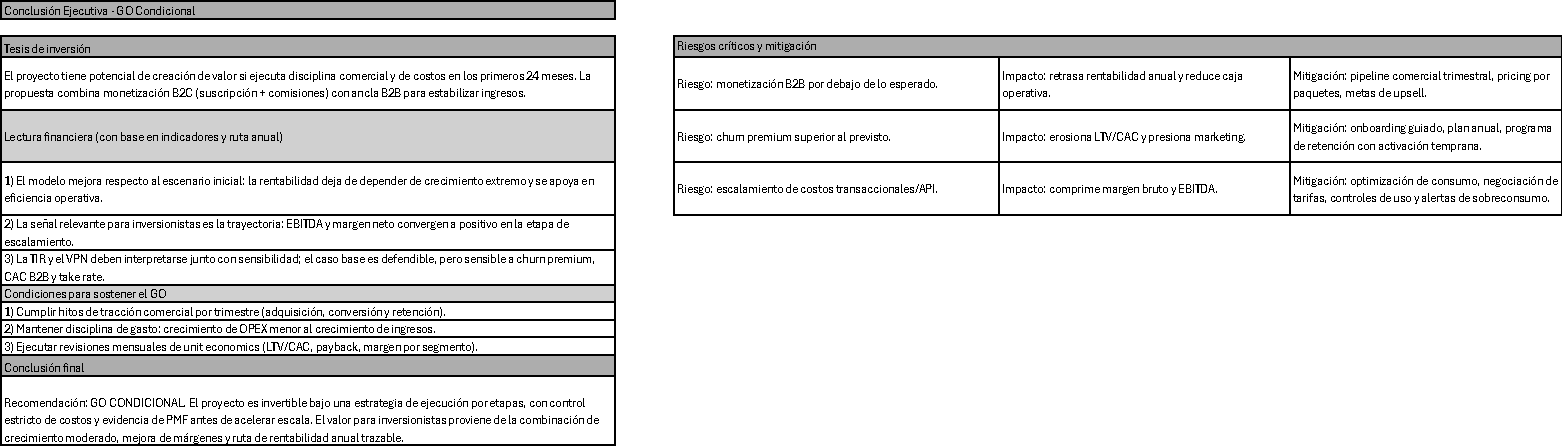
\includegraphics[width=\textwidth]{../assets/figures/finance.conclusion.pdf}
\caption{Análisis Final GO/NO GO y Recomendaciones Estratégicas}
\end{figure}

\textbf{Conclusión Final: GO CONDICIONAL}

Basado en el análisis detallado de riesgos y oportunidades, el modelo de negocio es \textbf{VIABLE} con ajustes críticos y ofrece una relación atractiva entre riesgo asumido y retorno potencial. La propuesta de valor es diferenciada (IA + red social + planificación), la oportunidad de mercado está alineada con la digitalización del turismo y la estructura tecnológica ya anticipa una operación capaz de escalar regionalmente. El GO está condicionado a:

\begin{enumerate}
    \item \textbf{VALIDAR} pricing premium y propuesta B2B con cohortes reales de adopción.
    \item \textbf{IMPLEMENTAR} control de costos transaccionales/API y observabilidad de margen por segmento.
    \item \textbf{ASEGURAR} runway suficiente para ejecutar fase de validación y fase de escalamiento.
    \item \textbf{DEFINIR} gobierno de IA y políticas de uso justo antes de expansión comercial.
\end{enumerate}

La oportunidad es especialmente interesante porque combina timing favorable, capacidad de diferenciación y espacio para expansión geográfica. Con capital suficiente y ejecución disciplinada, la plataforma puede pasar de una validación local a una base replicable para crecimiento regional, manteniendo el foco en eficiencia, control de margen y construcción de valor de largo plazo.

\end{document}
